\documentclass[a4paper,12pt]{article}
\usepackage{multirow}
\usepackage[icelandic]{babel}
\usepackage[T1]{fontenc}
\usepackage[utf8x]{inputenc}
\usepackage{graphicx}
\usepackage{fancyhdr}
\usepackage[top=1.4in, bottom=1.4in, left=1.2in, right=1.2in]{geometry}
\usepackage[T1]{fontenc}
\usepackage{textcomp}
\usepackage{gensymb}
\usepackage{pdflscape}
\usepackage[framed,numbered,autolinebreaks,useliterate]{mcode}\lstset{language=matlab} 
\lstset { inputencoding=latin1,
    language=python,backgroundcolor=\color{black!5}, % set backgroundcolor
    basicstyle=\ttfamily\footnotesize,
    keywordstyle=\color{blue}\bfseries,
    stepnumber=1,
    morekeywords={set,param,var,solve,data,display,maximize,minimize,subject to,sum}
}
\usepackage{caption}
\usepackage{here}
\usepackage{amsmath} % or simply amstext
\newcommand{\angstrom}{\textup{\AA}}
\usepackage{subcaption}
\usepackage{url} 
%\usepackage[table]{xcolor}
\usepackage[version=3]{mhchem}
\usepackage{layout}
\usepackage[parfill]{parskip}
\usepackage{arydshln}
\pagestyle{fancy}
\lhead{}
\chead{}
\rhead{IÐN401G \\ Vor 2014}
\lfoot{Háskóli Íslands}
\cfoot{}
\rfoot{\thepage}
\renewcommand{\headrulewidth}{0.0pt}
\renewcommand{\footrulewidth}{0.0pt}

\begin{document}
\begin{titlepage}
\begin{center}
\begin{minipage}{0.4\textwidth}
\begin{flushleft} 
\vspace{10mm}
        \begin{figure}[H]
      
\includegraphics[width=0.4\linewidth]{HI_merki.jpg}
        \label{fig: logo}
        \end{figure}
\end{flushleft}
\end{minipage}
\begin{minipage}{0.4\textwidth}
\begin{flushright} \large
\textsc{Háskóli Íslands\\Verkfræðideild}
\end{flushright}
\end{minipage}

\vspace{4cm}



%
\includegraphics[width=0.15\textwidth]{HI_merki.jpg}\\[1cm]


{\textsc{\Large Aðgerðagreining}\\[0.5cm]}

\vspace{0.8cm}
% Title
\begin{center}
\rule{1\textwidth}{3pt}

{\textsc{ \LARGE \bfseries Bestun stundatöflu í stokkakerfi}} \\[0.4cm]



\rule{1\textwidth}{4pt}
\vspace{2cm}

\end{center}
\today

\vfill

\begin{minipage}{0.4\textwidth}
\begin{flushleft} 
\vspace{1cm}
\emph{Kennari:}\\
\textsc{Tómas Philip Rúnarsson}\\
\end{flushleft}
\end{minipage}
\begin{minipage}{0.4\textwidth}
\begin{flushright} 
\emph{Nemendur:}\\
Baldur Geir Gunnarsson\\
Einar Halldórsson\\
Gestur Hvannberg\\
Oddur Vilhjálmsson\\
Trausti Kouichi Ásgeirsson
\end{flushright}
\end{minipage}
% Bottom of the page
%{\large Vorönn, 2014}

\end{center}

\newpage
\thispagestyle{empty} \mbox{}
\vfill
%\begin{center}\textit{\thesisdedication}\end{center} \vspace*{5cm}
\vfill 
\thispagestyle{empty}
\cleardoublepage



\end{titlepage}

\title{Bestun stundatöflu í stokkakerfi}
\author{Baldur Geir Gunnarsson, Einar Halldórsson, Gestur Hvannberg,\\ Oddur Vilhjálmsson, Trausti Kouichi Ásgeirsson}
\maketitle

\section{Ágrip}
Verkfræði og náttúruvísindasvið Háskóla Íslands notast við stokkakerfi við stundatöflugerð. Samtals eru 8 stokkar á hverri önn og raða þarf áföngum niður á þá. Samtals eru 7 stokkar á hverri önn og raða þarf áföngum niður á þá. Oftast eru 5 áfangar á önn sem er 6 einingar hver fyrir sig, samtals 30 einingar.Á myndinni má sjá 7 stokka en við nefndum stokk 8 fyrir alla áfangana sem lenda utan þessara stokka. Markmið okkar var að hanna stundatöflur fyrir allar annir í Eðlisfræði og kanna eiginleika þeirrar lausnar.
\begin{figure}[ht!]
\centering
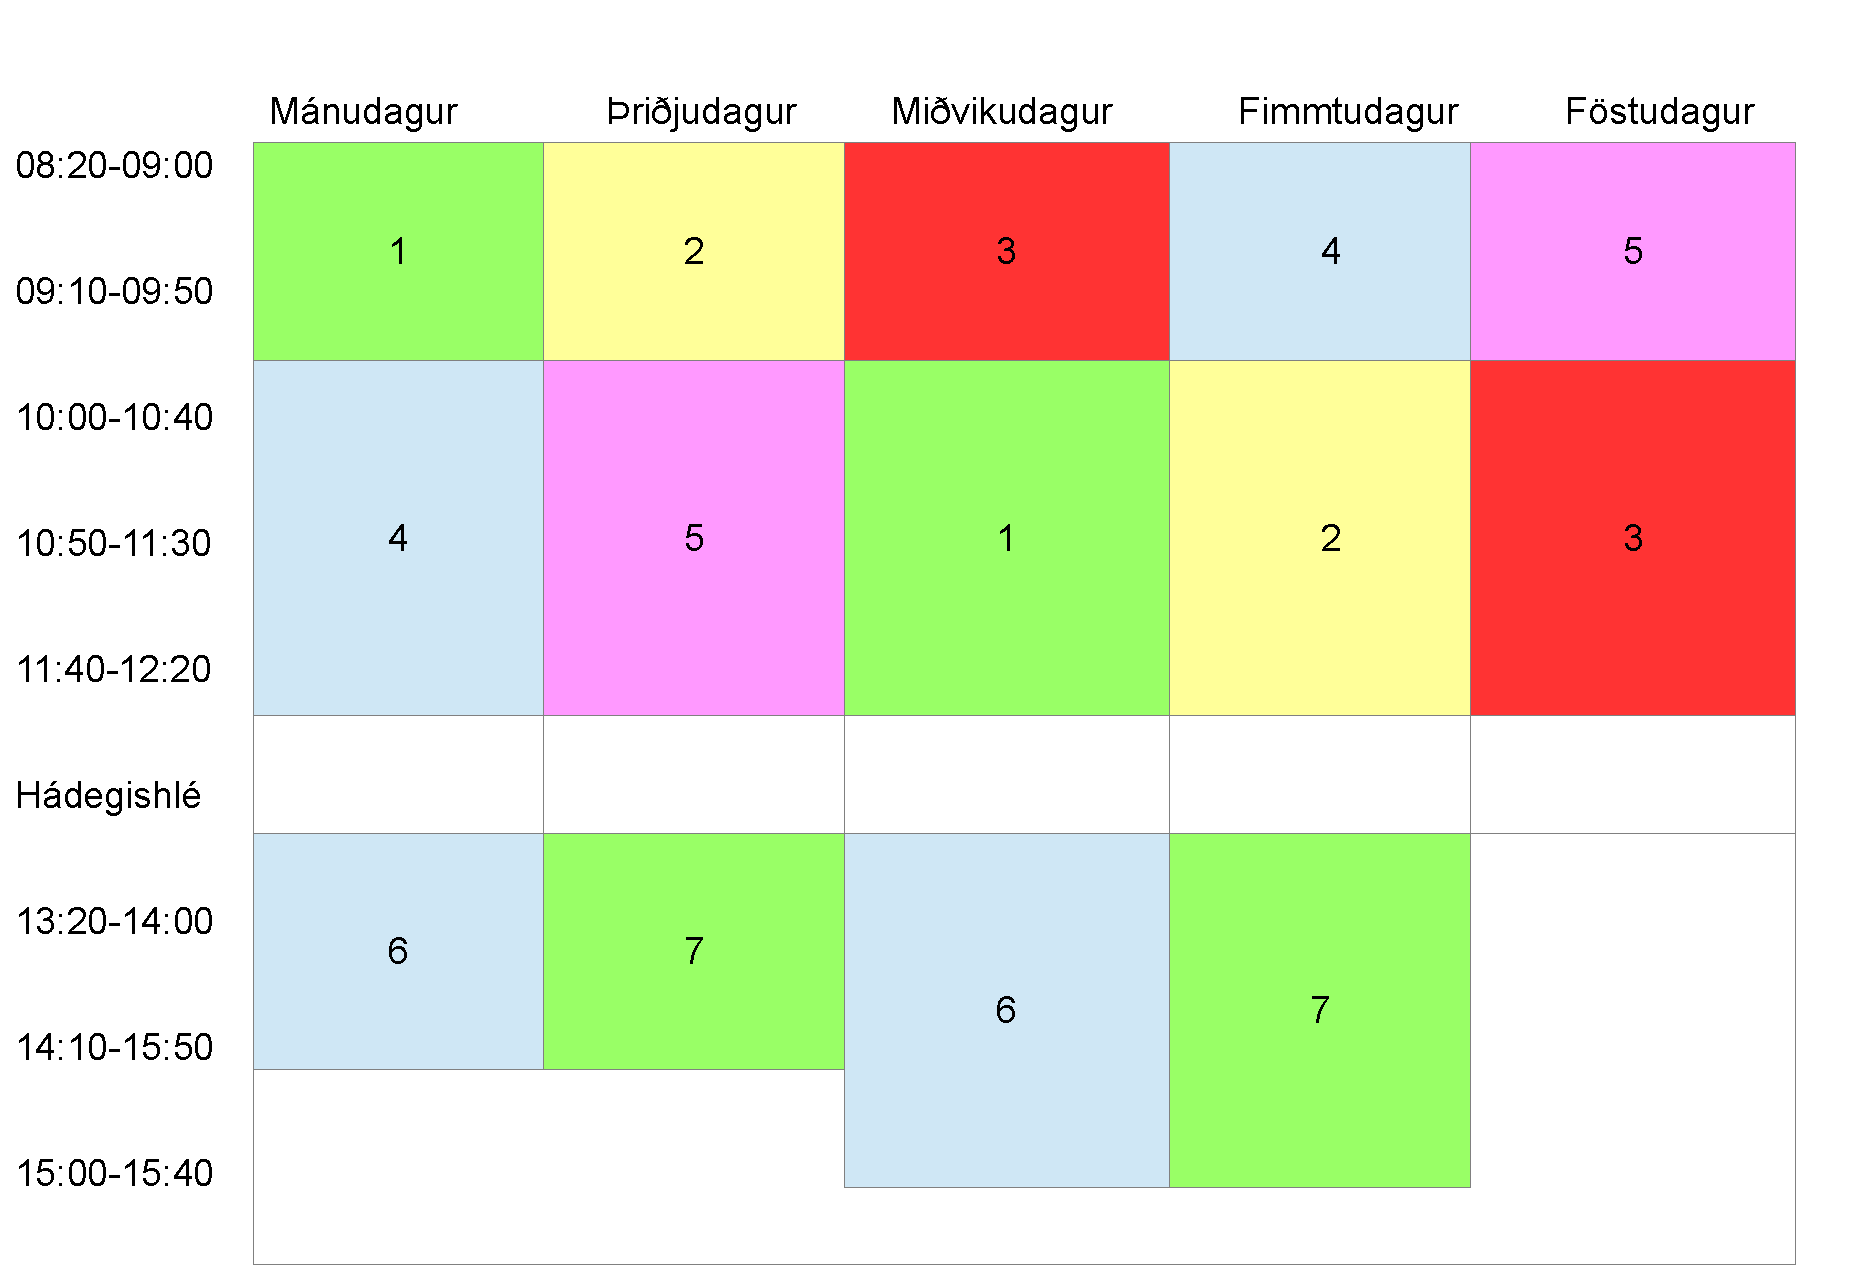
\includegraphics[scale=0.3]{stundatafla}
\caption{Stundatafla stokka}
\label{fig: stundatafla}
\end{figure}

Við nefndum svo stokk 8 þar sem áfangar raðast niður utan þessara stokka. Eftir að hafa gert líkan tókst að raða áföngum þannig að þeir tóku bara 1 stokk hver. Gefin var skrá með lista á 1858 nemendur og hvaða námskeið þeir völdu. Við bjuggum til forrit sem raðar nemendum upp í æskilega stokka eftir þeim námskeiðum sem þeir velja og reynum að forðast árekstra en því miður þá eru oftast eitthverjir sem lenda í árekstri við önnur fög innan stokksins. Forritið sem við skrifuðum les úr gögnunum sem voru gefin og raðar í stokka. Forritið gefur góða lausn sem hentar eðlisfræðinni vel.




\section{Inngangur/bakgrunnur}
Í þessu verkefni eigum við að raða nemendum sem eru að læra eðlisfræði í ákveðna stokka (mynd 1) eftir námskeiðum sem þeir velja. Gefin er .dat skrá með lista yfir 1858 nemendur sem eru skráðir á verkfræði og náttúruvísindasvið Háskóla Íslands og í þessari sömu skrá er listi yfir 141 námskeið sem eru í boði. Við reynum að láta verklega tíma, dæmatíma og æfingatíma falla utan við stokka (stokkur 8). Hvert námskeið fær tvo daga í viku, annan daginn eru tímarinr 2 x 40 mínútur og hinn daginn 3 x 40 mínútur.
Stundatöflur fyrir núverandi vormisseri samræmast ekki fyrirfram skilgreindum kennslustokk samkvæmt kennsluskrá. Eitt af okkar verkefnum er að láta stundatöflurnar vera einsleitar frá ári til árs og þá sérstaklega fyrir fyrsta árið. Erfitt era ð gera góða stundatöflu fyrir annað og þriðja ár því þá fara val áfangar að koma inn og jafnvel endurtekning námskeiða eftir fall.
Við höfum engin áhrif á hvernig námskeið utan eðlisfræðinnar er raðað í stundatöflunni en áhugavert er að sjá hversu tengdar allar 15 námsleiðirnar eru. Á mynd 2 má sjá fylgni námsleiða eftir vali nemenda við viðkomandi námsleið.


\begin{figure}[ht!]
\centering
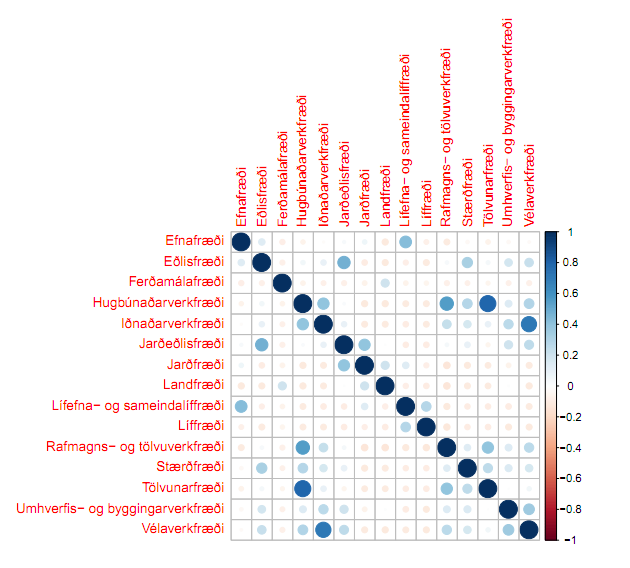
\includegraphics[scale=0.6]{thyrping}
\caption{Fylgni milli námskeiða}
\label{fig: thyrping}
\end{figure}
\pagebreak

Við stundatöflugerð er nauðsynlegt að við forgangsröðum áföngum rétt, þ.e.a.s að skyldunámskeið á ákveðnum misserum stangist ekki við önnur skyldunámskeið. Námskeið sem mega ekki lenda í sama stokki mynda námskeiðshóp. Nemendur mynda þessa námskeiðshópa út frá skráningu þeirra í námskeið. Ef námskeið eru skylda þá munu þau vafalaust vera valin af nemendum og skyldunámskeiðshópar þannig myndaðir sjálfkrafa. Eini gallinn er samt að námskeiðshópar sem eru með fáa nemendur geta lent í árekstri. Mikilvægt er að öll gögn séu rétt til að gefa rétta mynd af stöðu mála. 

\section{Niðurstöður, niðurlag og tillögur}

\begin{figure}[ht!]
\centering
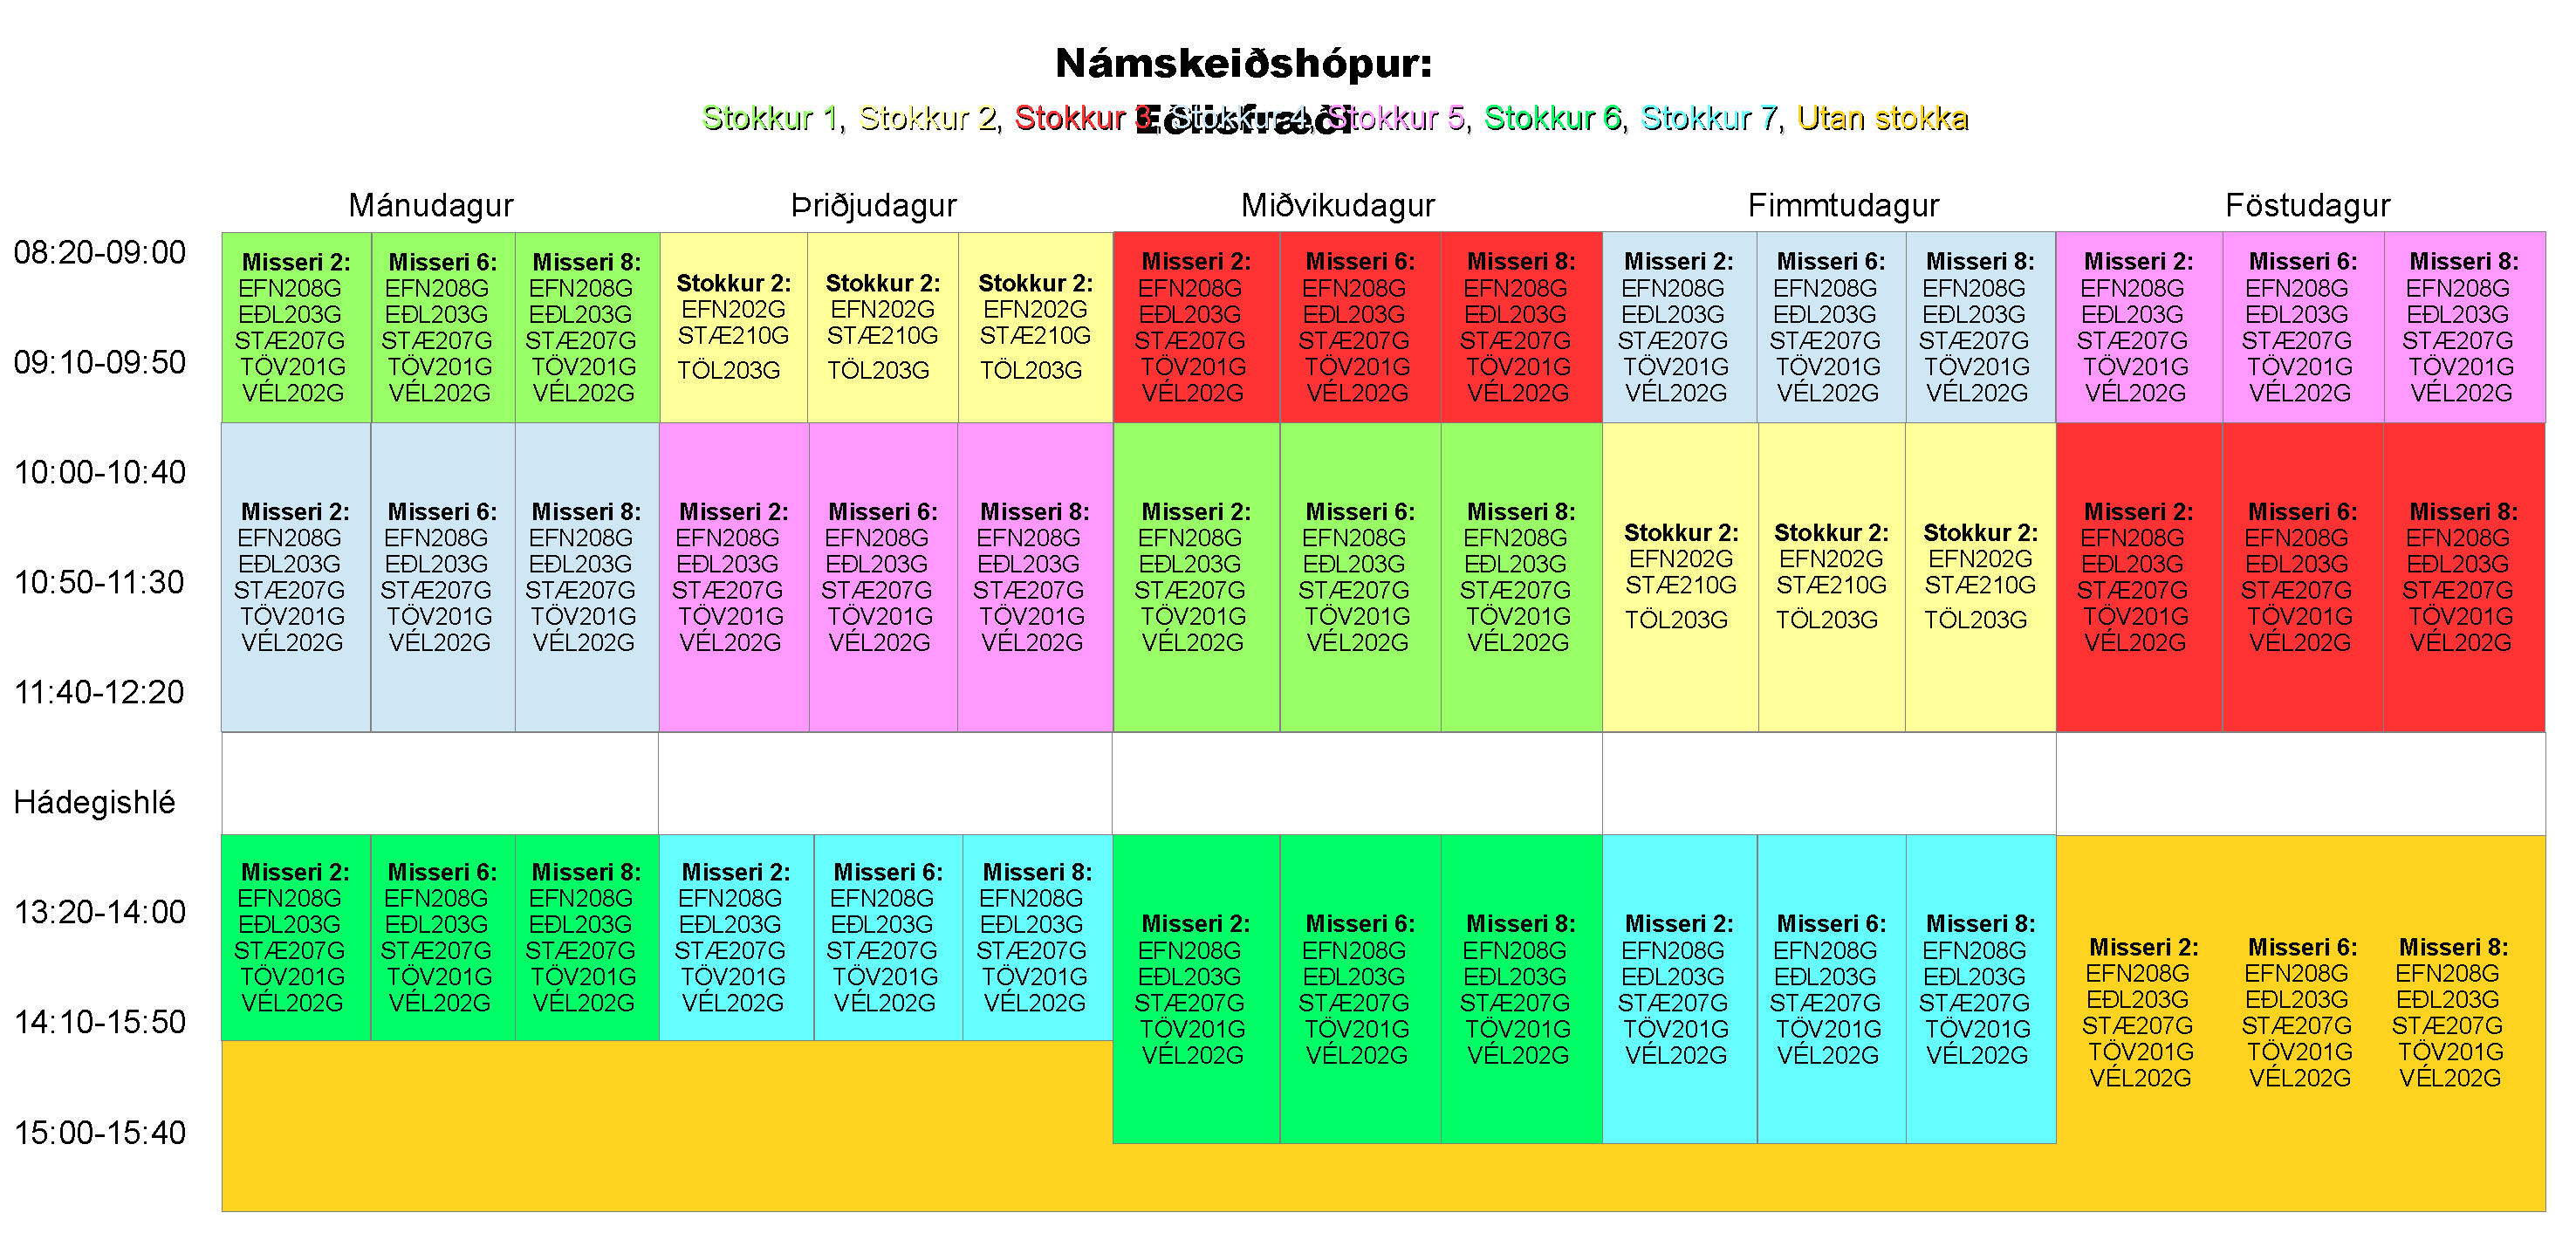
\includegraphics[width=120mm]{stundatoflur}
\caption{Röðun námskeiða í stundatöflur fyrir allar vorannir}
\label{fig: stundatoflur}
\end{figure}



Byrjuðum á því að setja þá skorðu að hvert námskeið sé kennt aðeins einu sinni og hver stokkur taki að hámarki 5 kennslustundum samtals nema stokkur 8 sem getur tekið við afgangstímum. Pössuðum upp á að eitt námskeið við námskeiðshóp væri kennt í einu svo nemendur í þeim hópum lentu ekki í árekstrum. Lögleg lausn fannst á þessu keyrsluforriti.

Markfalli var svo bætt við sem hámarkaði fjölda námskeiða í stokki 1-5 og lágmarkaði þá sem lenda þeirra stokka, eða þeirra sem væru eftir hádegi. Samkvæmt þessu ættu 10 áfangar að vera eftir hádegi.

c) tölfræði árekstra, hvers eðlis eru árekstrarnir fyrir Eðlisfræðina, núverandi stundatöflur fyrir vormisseri, bæta við fleiri námskeiðshópum?......bæta við og leysa aftur


Sjáum hér á grafi fyrir neðan að langflestir árekstrar myndast í stokki 5 eða um 37$\%$. 


\begin{figure}[ht!]
\centering
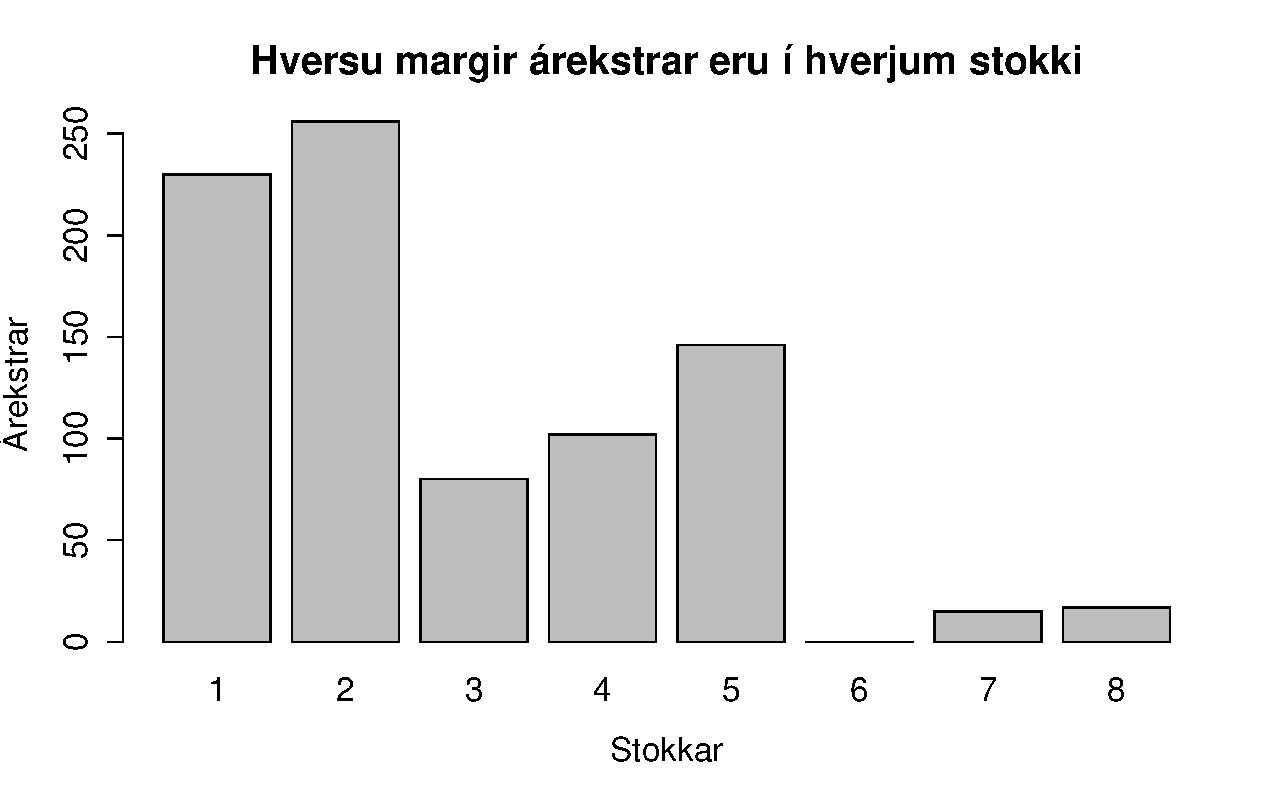
\includegraphics[width=120mm]{c_lidur_plot}
\caption{Árekstrar í hverjum stokk}
\label{fig: arekstrar}
\end{figure}



d)

Fjöldi námskeiða sem lenda í æskilegum stokk eða stokkum 1-5 á hverju misseri fyrir sig sig:

Æskileg skipting á misseri 2 = 18\\
Æskileg skipting á misseri 4 = 28\\
Æskileg skipting á misseri 6 = 17

Núna eru 14 áfangar eftir hádegi sem er aukning um 4. Því er í raun verra að nota fyrifram skilgreinda stokka samkvæmt þessu.

e)kennslustofunýting, námskeið fyrir hádegi


Til að stofunýting sé sem best skrifuðum við kóða sem lágmarkar tómar skólastofur

f)besta útfærsla stundatöflu....heildarfjöldi árekstra

\section{Aðferðir}
frásögn þannig að annar nemandi skilji það og að aðrir geti í
grundval laratriðum endurtekið niðurstöðurnar
\begin{itemize}
\item Fræði
\item Tækni
\item Greining
\item Reiknirit
\end{itemize}


Almennt línulegt bestunarlíkan er þar sem gefið er:

Hráefni(e.resources) með takmörkuðu framboði  $b_i$, á hráefni i þar sem:
\[i=1,....,m\]
Framleiðsluvörur(e.activities), ákvarðað er $x_j$ sem er framleitt magn eininga af vöru j þar sem:
\[j=1,....,m\]
Hagnaður $c_j$ af hverri einingu j. 

Notkun hráefnis i í vöru j þar sem $a_{ij}$.

Verkefnið er að hámarka(eða lágmarka):
\[max_{x1,.....,xn}Z = \sum_{j=1}^{n}c_j x_j\]
með skorðum i=1,...,m.
\[\sum_{j=1}^{n}a_{ij} x_j\leq b_i\]
\[x_j\geq 0, j=1,....,n\]
Fylkjaform:
\[max_xZ=c^Tx\]
með skorðum:
\[Ax\leq b\]
\[x\geq 0\]
Byrjum á því að setja verkefnið okkar upp í gusek með gefnum mengjum og breytum:
\lstinputlisting{almennt.mod}
Þar á eftir skilgreingum við ákvörðunarbreytunar V[n,s], námskeiðið sé kennt aðeins einu sinnu og að 
hver stokkur taki að hámarki við 5 kennslustundum (nema stokkur 8).

\lstinputlisting{stundatoflugerd2.mod}
Til að hámarka fjölda námskeiða sem lenda í stokki 1-5 bætum við eftirfarandi skorðu við:
\lstinputlisting{blidur.mod}
Því næst þurfum við að skoða árekstrana sem myndast
\lstinputlisting{clidur.mod}



\section{Almenn umfjöllun....sleppa??}
\begin{itemize}
\item Skyld verkefni
\item Skyld rit
\item Aðrar leiðir sem hafa ekki verið prófaðar
\end{itemize}




\pagebreak

\addcontentsline{toc}{section}{Heimildir}
\begin{thebibliography}{2}
	\bibitem{b:vs} Vinnuseðill í Aðgerðagreiningu (IÐN401G) , \textit{Bestun stundatöflu í stokkagerð, Tómas Philip Rúnarsson, Vorönn 2014}. 
	\bibitem{b:vs} Linear Programming: Foundations and Extensions , \textit{Robert J. Vanderbei, 2008}. 
\end{thebibliography}


\pagebreak
\section{Viðauki}
\textbf{b)} \\
\lstinputlisting{stundatoflugerd.mod}

má setja á tölvudisk með góðum útskýringum
\begin{itemize}
\item Stærðfræðileg líkön
\item Flæðirit
\item Gögn
\item Stórar töflur með niðurstöðum
\end{itemize}

\end{document}


